% Copyright 2004 by Till Tantau <tantau@users.sourceforge.net>.
%
% In principle, this file can be redistributed and/or modified under
% the terms of the GNU Public License, version 2.
%
% However, this file is supposed to be a template to be modified
% for your own needs. For this reason, if you use this file as a
% template and not specifically distribute it as part of a another
% package/program, I grant the extra permission to freely copy and
% modify this file as you see fit and even to delete this copyright
% notice. 

\documentclass{beamer}
\usepackage{tikz}
\usetikzlibrary{trees}
\usepackage[ngerman]{babel}
\usepackage[utf8]{inputenc}
\usepackage{graphics}
\usetikzlibrary{positioning}
\usepackage[decimalsymbol=comma]{siunitx}
\usepackage{amsmath}
\usepackage{ziffer}
\usepackage{scrextend}
\usepackage{color, colortbl}
\usepackage{ulem}
\usepackage{multicol}
\usepackage{qrcode}
\usepackage{listings}
\usepackage{minted}
\usepackage[export]{adjustbox}




% There are many different themes available for Beamer. A comprehensive
% list with examples is given here:
% http://deic.uab.es/~iblanes/beamer_gallery/index_by_theme.html
% You can uncomment the themes below if you would like to use a different
% one:
%\usetheme{AnnArbor}
%\usetheme{Antibes}
%\usetheme{Bergen}
%\usetheme{Berkeley}
%\usetheme{Berlin}
%\usetheme{Boadilla}
%\usetheme{boxes}
%\usetheme{CambridgeUS}
%\usetheme{Copenhagen}
%\usetheme{Darmstadt}
\usetheme{default}
%\usetheme{Frankfurt}
%\usetheme{Goettingen}
%\usetheme{Hannover}
%\usetheme{Ilmenau}
%\usetheme{JuanLesPins}
%\usetheme{Luebeck}
%\usetheme{Madrid}
%\usetheme{Malmoe}
%\usetheme{Marburg}
%\usetheme{Montpellier}
%\usetheme{PaloAlto}
%\usetheme{Pittsburgh}
%\usetheme{Rochester}
%\usetheme{Singapore}
%\usetheme{Szeged}
%\usetheme{Warsaw}

\newcommand*\conj[1]{\overline{#1}}
\newcommand*\oo{\infty}

\definecolor{tucinfo}{rgb}{0.49,0.6,0.16}
\definecolor{LightCyan}{rgb}{0.88,1,1}
\definecolor{Blue}{rgb}{0,0,1}

\setbeamercolor{title}{fg=Blue}
\setbeamercolor{structure}{fg=Blue}


\title{ansible-tine}

% A subtitle is optional and this may be deleted
\subtitle{out of the box mailserver, crm, cms solution}

\author{Stefan Helmert}
% - Give the names in the same order as the appear in the paper.
% - Use the \inst{?} command only if the authors have different
%   affiliation.

\institute[Entroserv] % (optional, but mostly needed)
{
	\url{https://www.entroserv.de/de/offene-software/ansible-tine}
}


% - Use the \inst command only if there are several affiliations.
% - Keep it simple, no one is interested in your street address.

\date{20.04.2019}
%\date{\today}
% - Either use conference name or its abbreviation.
% - Not really informative to the audience, more for people (including
%   yourself) who are reading the slides online

\subject{Cryptdomainmgr}
% This is only inserted into the PDF information catalog. Can be left
% out. 

% If you have a file called "university-logo-filename.xxx", where xxx
% is a graphic format that can be processed by latex or pdflatex,
% resp., then you can add a logo as follows:

% \pgfdeclareimage[height=0.5cm]{university-logo}{university-logo-filename}
% \logo{\pgfuseimage{university-logo}}
\logo{\large{EH19}}

% Delete this, if you do not want the table of contents to pop up at
% the beginning of each subsection:
%\AtBeginSubsection[]
%{
%  \begin{frame}<beamer>{Inhalt}
%    \tableofcontents[currentsection,currentsubsection]
%  \end{frame}
%}

% Let's get started
\begin{document}
	
	\begin{frame}
		\titlepage
	\end{frame}
	
	\begin{frame}{Content}
		%\begin{multicols}{2}
		\tableofcontents
		%\end{multicols}
		% You might wish to add the option [pausesections]
	\end{frame}
	
	% Section and subsections will appear in the presentation overview
	% and table of contents.
	\pagenumbering{arabic}
	
	\section{Motivation}
	\begin{frame}{\insertsection}{\insertsubsection}
		\textbf{$\rightarrow$ let's run a startup company $\leftarrow$}\\
		\textbf{We need:}
		\begin{itemize}
			\item Webpage (CMS)
			\item E-Mail (Mailserver, Spamfilter)
			\item Mailinglist
			\item Groupware, CRM
			\item \textbf{and the s for security}
		\end{itemize}
	\end{frame}
	
	\section*{DeMotivation}
	\begin{frame}{\insertsection}{\insertsubsection}
		\vspace{-0.5cm}
		\textbf{$\rightarrow$ let's run a startup company $\leftarrow$}\\
		\textbf{IT-Infrastructure:}
		\begin{itemize}
			\item Cloud Solution
			\begin{itemize}
				\item DSGVO?
				\item Lock-In?
				\item Security?
				\item price?
			\end{itemize}
			\item Self-Hosted
			\begin{itemize}
				\item Installation?
				\item Configuration?
				\item Updates?
				\item Backups?
				\item Documentation?
				\item Will it work?
			\end{itemize}
			\item Self-Hosted using integrated solution
			\begin{itemize}
				\item everything fully supported?
				\item price?
			\end{itemize}
			\item Dedicated-Hosting by IT-Service
			\begin{itemize}
				\item price?
			\end{itemize}
		\end{itemize}
	\end{frame}
	
\section{We need}
	\begin{frame}{\insertsection}{\insertsubsection}
		\vspace{-0.5cm}
		
		\dots to get ready \textbf{NOW}
		
		\begin{itemize}
			\item \textbf{self-hosted} but:
			\item easy to install
			\item easy to configure
			\item easy to integrate
			\item useful defaults 
		\end{itemize}
		$\rightarrow$ Fill out form and click \textbf{START}
	\end{frame}

	\begin{frame}{\insertsection}{\insertsubsection}
		\vspace{-0.5cm}
		
		\dots useful \textbf{TOOLS} and \textbf{FEATURES}
		
		\begin{itemize}
			\item E-Mail (Webmail, SMTP, IMAP, Exchange)
			\item Default signature
			\item Multiuser + Frontend for administration
			\item Mail-Alias
			\item Quota
			\item Sieve integration
			\item Spamfilter with Learning (integrated in Mailclient) 
			\item Autoconfig (Thunderbird), Autodiscovery (ActiveSync)
			\item Calendar (Web, Caldav and ActiveSync)
			\item Addressbook (synced)
			\item Mailinglist
			\item TLS, TLSA, DKIM, DMARC, SPF, ADSP, ARC
			\item Filestorage
			\item Backup
			\item Flatfile CMS
		\end{itemize}

	\end{frame}

	\begin{frame}{\insertsection}{\insertsubsection}
		\vspace{-0.5cm}
		
		\dots some nice to have tools
		
		\begin{itemize}
			\item Human Resource Management
			\item CRM
			\item Timekeeping
			\item Base data
			\item Sales
			\item Task Planning
			\item Inventory management
		\end{itemize}
		
	\end{frame}

\section{Components}
	\begin{frame}{\insertsection}{\insertsubsection}
		\vspace{-0.5cm}
		
		\begin{itemize}
			\item Tine 2.0
			\item Apache2
			\item Postfix
			\item Dovecot
			\item Sieve
			\item MySQL/Mariadb
			\item Rspamd
			\item Mailman
			\item Cryptdomainmgr (+ dehydrated)
			\item Cron
			\item Ansible
			\item inwx.de
			\item Letsencrypt
			\item Grav
		\end{itemize}
	\end{frame}

	\begin{frame}{\insertsection}{\insertsubsection}
		\vspace{-0.5cm}
		
		\begin{itemize}
			\item Tine 2.0
			\begin{itemize}
				\item Accountmanagement, Administration
				\item ActiveSync, Exchange
				\item Caldav
				\item Carddav
				\item Groupware, CRM and additional tools
				\item Webmail
				\item Filestorage
			\end{itemize}
			\item Apache2
			\begin{itemize}
				\item Web-UIs
				\item Webpage
				\item PHP
				\item TLS
			\end{itemize}			
			\item Postfix
			\begin{itemize}
				\item SMTP
			\end{itemize}			
			\item Dovecot
			\begin{itemize}
				\item IMAP
			\end{itemize}
			\item Sieve
			\begin{itemize}
				\item Filtering
				\item Control remote spam/ham learning
			\end{itemize}
		\end{itemize}
	\end{frame}
	
	\begin{frame}{\insertsection}{\insertsubsection}
		\vspace{-0.5cm}
		
		\begin{itemize}
			\item MySQL/Mariadb
			\begin{itemize}
				\item Store Useraccounts
				\item Store Mailaccounts
			\end{itemize}
			\item Rspamd
			\begin{itemize}
				\item Spamcheck
				\item DKIM signing
				\item DKIM keygen
			\end{itemize}
			\item Mailman
			\begin{itemize}
				\item Mailinglist
				\item Mailinglist administration
			\end{itemize}
			\item Cryptdomainmgr (+ dehydrated)
			\begin{itemize}
				\item TLS certificates
				\item TLSA
				\item DKIM
				\item Domain management (update records)
				\item DH params
			\end{itemize}
			\item Cron
			\begin{itemize}
				\item Used by Tine 2.0 and Cryptomainmgr
			\end{itemize}
			\item Ansible
			\begin{itemize}
				\item Install and configure all this
			\end{itemize}

		\end{itemize}
	\end{frame}
	
	\begin{frame}{\insertsection}{\insertsubsection}
		\vspace{-0.5cm}
		
		\begin{itemize}
			\item inwx.de
			\begin{itemize}
				\item hosts domain
				\item controlled by Cryptdomainmgr
				\item DNSSEC
			\end{itemize}
			\item Letsencrypt
			\begin{itemize}
				\item Provides TLS certificates
			\end{itemize}
			\item Grav
			\begin{itemize}
				\item Webpage/CMS
			\end{itemize}
		\end{itemize}
	\end{frame}
	
\section{Getting started}
\subsection{Domain}
\begin{frame}{\insertsection}{\insertsubsection}
	\vspace{-0.5cm}
	Currently only Internetworx (\url{inwx.de}) supported;\\
	No reseller support yet 
	\begin{itemize}
		\item create account
		\begin{itemize}
			\item username and password for automatic update needed
			\item individual account for client required
		\end{itemize}
		\item register domain
	\end{itemize}
\end{frame}	

\subsection{Server}
\begin{frame}{\insertsection}{\insertsubsection}
	\vspace{-0.5cm}
	Smallest V-Server (1 GB RAM, 50 GB SSD)
	\begin{itemize}
		\item install full Server Ubuntu 18.04 or Debian 9
		\item enable SSH root access
	\end{itemize}
\end{frame}	

\subsection{Deploy}
\begin{frame}[fragile]{\insertsection}{\insertsubsection}
	\vspace{-0.5cm}
	\textbf{Config -- CRM, email}\\
	vars/common.yml
    \begin{minted}[gobble=2,frame=single,linenos]{yaml}
		hostname: "pserver"
		tld: "entroserv.de"
		subdomain: "{{ tld }}"
		servername: "pserver"
		domain: "{{ servername }}.{{ subdomain }}"
		tinedomains:
		  - "tine20.{{ subdomain }}"
		rspamddomains:
		  - "rspamd.{{ subdomain }}"
		emaildomain: "{{ subdomain }}"
		imapuserdomain: "entro"
		tlsa: 'auto:3:1:1,auto:2:0:1'
	\end{minted}
\end{frame}	

\begin{frame}[fragile]{\insertsection}{\insertsubsection}
	\vspace{-0.5cm}
	\textbf{Config -- Mailinglist}\\
	vars/common.yml
	\begin{minted}[gobble=2,frame=single,linenos]{yaml}
		defaultlistmap:
		         { emaildomain: "lists.{{ subdomain }}",
		             webdomain: "www.lists.{{ subdomain }}",
		                    mx: '{{ subdomain }}' }
	\end{minted}
\end{frame}	

\begin{frame}[fragile]{\insertsection}{\insertsubsection}
	\vspace{-0.5cm}
	\textbf{Config -- CMS, web}\\
	vars/common.yml
	\begin{minted}[gobble=2,frame=single,linenos]{yaml}
		webdomains: 
		  - "www.{{ subdomain }}"
		  - "{{ subdomain }}"
		grav_admin_user: "admin"
		grav_admin_email:
		        "{{ tine20_admin_name }}@{{ emaildomain }}"
	\end{minted}
\end{frame}	

\begin{frame}[fragile]{\insertsection}{\insertsubsection}
	\vspace{-0.5cm}
	\textbf{Config -- multidomain}\\
	vars/common.yml
	\begin{minted}[gobble=2,frame=single,linenos]{yaml}
		emailmaps:
		  - { emaildomain: "entroserv.net",
		               mx: "{{ domain }}" }
		  - { emaildomain: "entroserv.com",
		               mx: "{{ domain }}" }
		listmaps:
		  - { emaildomain: "lists.entroserv.net",
		        webdomain: "www.lists.entroserv.net",
		               mx: '{{ domain }}' }
		  - { emaildomain: "lists.entroserv.com",
		        webdomain: "www.lists.entroserv.com",
		               mx: '{{ domain }}' }
	\end{minted}
\end{frame}	

\begin{frame}[fragile]{\insertsection}{\insertsubsection}
	\vspace{-0.5cm}
	\textbf{Config -- TLS certificate}\\
	vars/cert.yml
	\begin{minted}[gobble=2,frame=single,linenos]{yaml}
		certemail: "stefan.helmert@t-online.de"
		certextra: []
		certocsp:
		  - "--ocsp"
		certbaselocation: "/etc/ssl"
	\end{minted}
\end{frame}	

\begin{frame}[fragile]{\insertsection}{\insertsubsection}
	\vspace{-0.5cm}
	\textbf{Config -- internetworx login}\\
	vars/inwx.yml
	\begin{minted}[gobble=2,frame=single,linenos]{yaml}
		inwxlogin: "entroserv"
	\end{minted}
	
	\textbf{Config -- internetworx password}\\
	vars/inwx.yml
	\begin{minted}[gobble=2,frame=single,linenos]{yaml}
		inwxpasswd: "**********"
	\end{minted}
\end{frame}	

\begin{frame}[fragile]{\insertsection}{\insertsubsection}
	\vspace{-0.5cm}
	\textbf{Config -- all passwords}\\
	vars/passwords.yml
	\begin{minted}[gobble=2,frame=single,linenos]{yaml}
		rspamd_pw: "{{  lookup('password', 'credentials/'
		              + inventory_hostname
		              + '/rspamd_pw.txt chars=ascii_letters,
		                                      digits') }}"
		[...]
	\end{minted}
\end{frame}	

\begin{frame}[fragile]{\insertsection}{\insertsubsection}
	\vspace{-0.5cm}
	\textbf{Start Ansible-Playbook}\\
	\begin{minted}[gobble=2,frame=single,linenos]{bash}
		ansible-playbook deploy_playbook.yml -i hosts
	\end{minted}
	
	\begin{verbatim}
	PLAY [crm-server] *********************************
	
	TASK [up : Debug host] ****************************
	ok: [92.60.36.246 -> localhost] => {
	    "msg": "92.60.36.246"
	}
	
	TASK [up : Waiting for startup] *******************
	ok: [92.60.36.246 -> localhost]
	\end{verbatim}
\end{frame}

\subsection{Setup}
\begin{frame}[fragile]{\insertsection}{\insertsubsection}
	\vspace{-0.5cm}
	Get tine20 admin password
	\begin{minted}[gobble=2,frame=single,linenos]{bash}
		cat credentials/92.60.36.246/tine20_admin_passwd.txt
	\end{minted}
	Login\\
	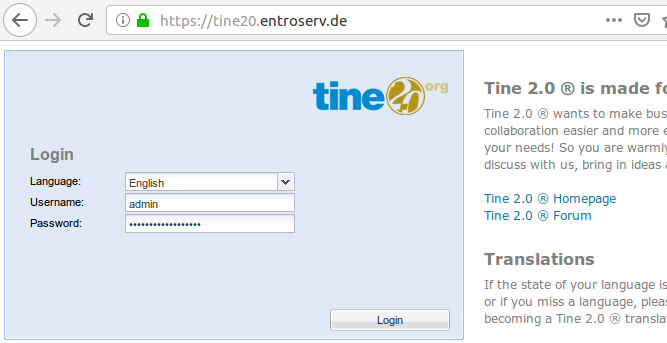
\includegraphics[width=10.5cm]{tine20login.png}
\end{frame}	

\begin{frame}[fragile]{\insertsection}{\insertsubsection}
	\vspace{-0.5cm}
	Add user\\
	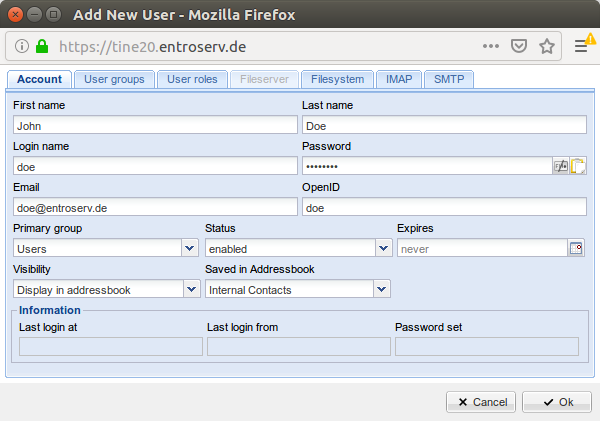
\includegraphics[width=9cm]{tine20adduser.png}\\
	\textbf{Important:} User must login and relogin to use email.
\end{frame}	

\begin{frame}[fragile]{\insertsection}{\insertsubsection}
	\vspace{-0.5cm}
	ActiveSync autodiscovery on Android\\
	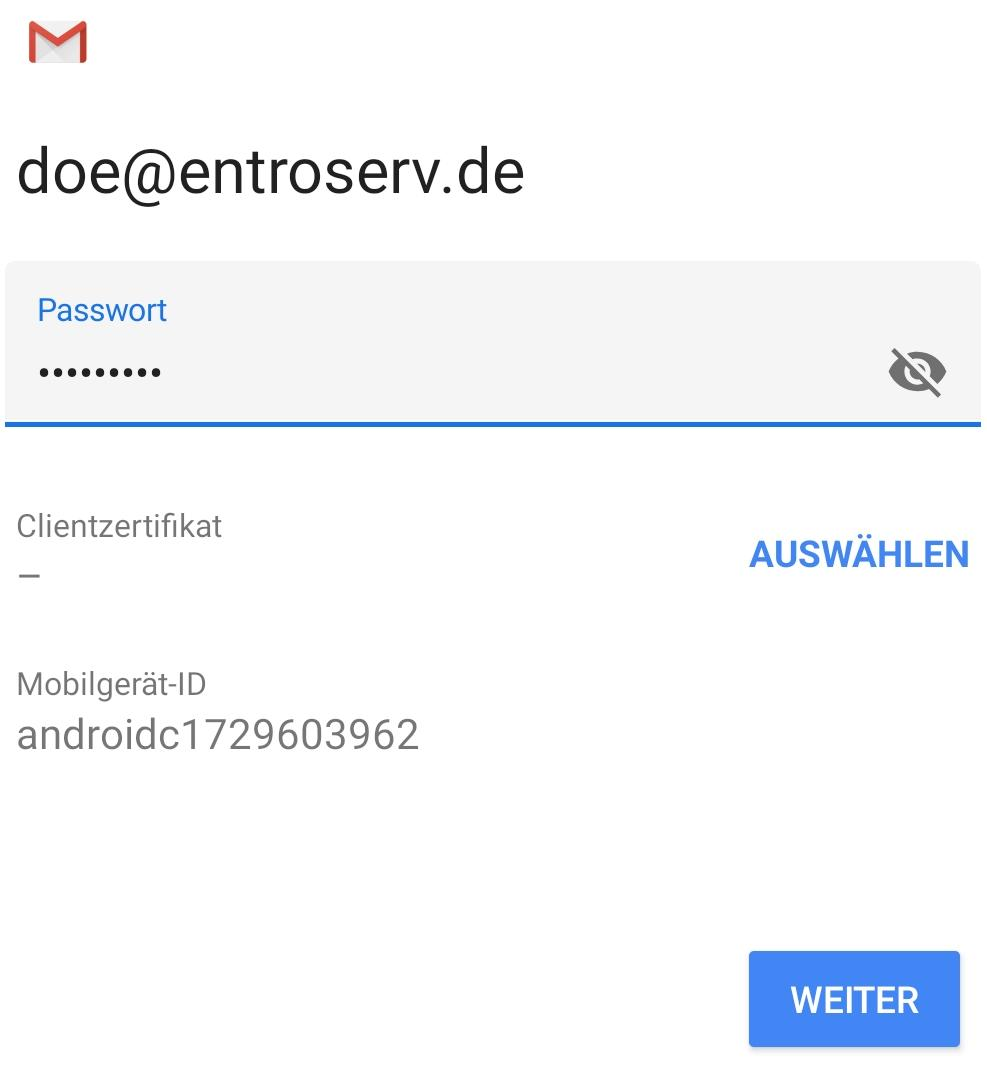
\includegraphics[width=3.5cm,valign=t]{autodiscoverAndroid1.jpg}
	
\includegraphics[width=3.5cm,valign=t]{autodiscoverAndroid2.jpg}
	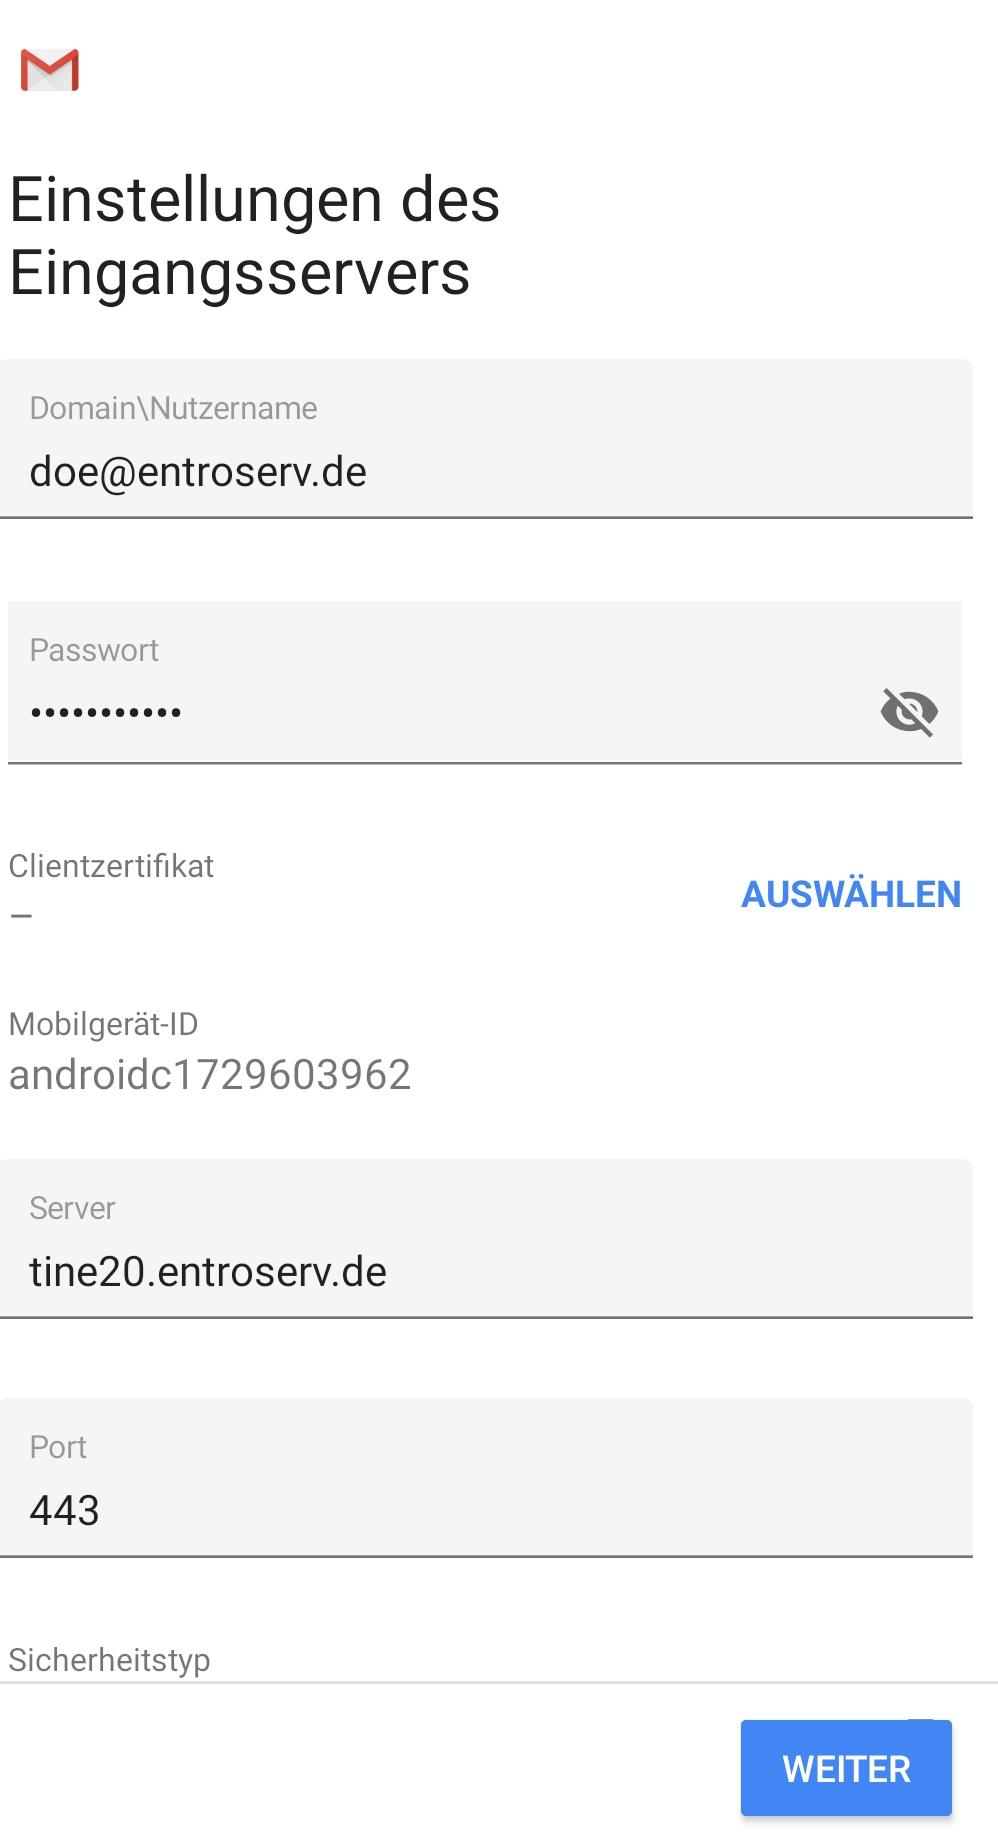
\includegraphics[width=3.5cm,valign=t]{autodiscoverAndroid3.jpg}

	\textbf{Because:} \url{https://autodiscover.entroserv.de/autodiscover/autodiscover.php}
\end{frame}	

\begin{frame}[fragile]{\insertsection}{\insertsubsection}
	\vspace{-0.5cm}
	IMAP/SMTP autoconfig for Thunderbird\\
	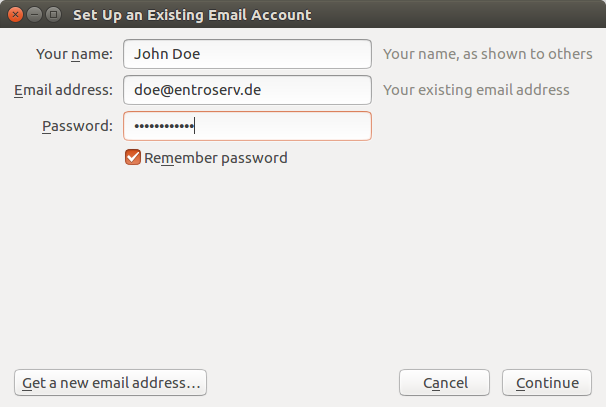
\includegraphics[width=9cm]{autoconfigTB1.png}\\
\end{frame}	

\begin{frame}[fragile]{\insertsection}{\insertsubsection}
	\vspace{-0.5cm}
	After $<1$ s\\
	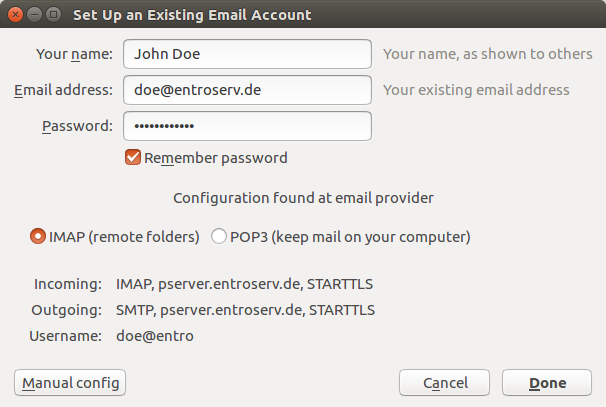
\includegraphics[width=9cm]{autoconfigTB2.png}\\
	\textbf{Because:} \url{https://autoconfig.entroserv.de/mail/config-v1.1.xml}
\end{frame}	

\begin{frame}[fragile]{\insertsection}{\insertsubsection}
	\vspace{-0.5cm}
	Calendar setup in Tine2.0
	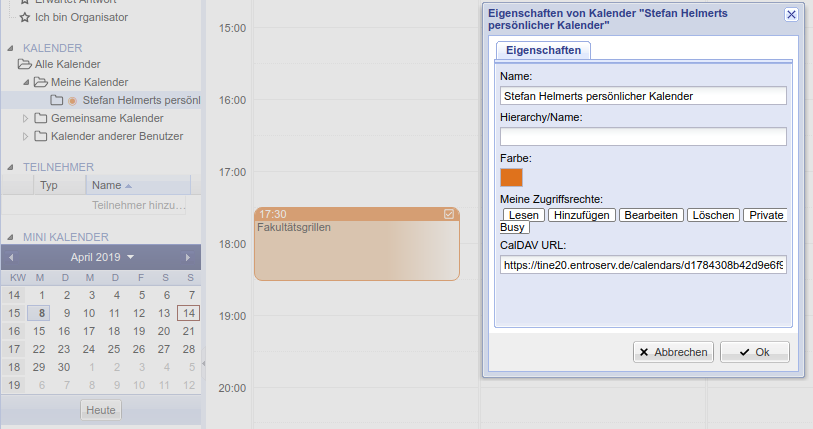
\includegraphics[width=11cm]{tine20Calendar.png}\\
\end{frame}	

\begin{frame}[fragile]{\insertsection}{\insertsubsection}
	\vspace{-0.5cm}
	CalDav in Thunderbird
	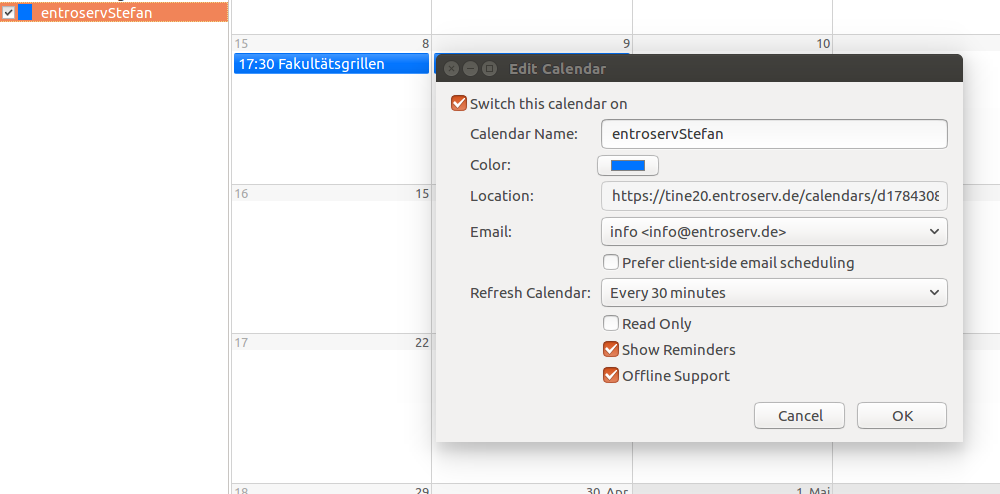
\includegraphics[width=11cm]{CalDavTB.png}\\
	Is there CalDav autoconfig available?
\end{frame}	

\begin{frame}[fragile]{\insertsection}{\insertsubsection}
	\vspace{-0.5cm}
	Adminpanel of mailman
	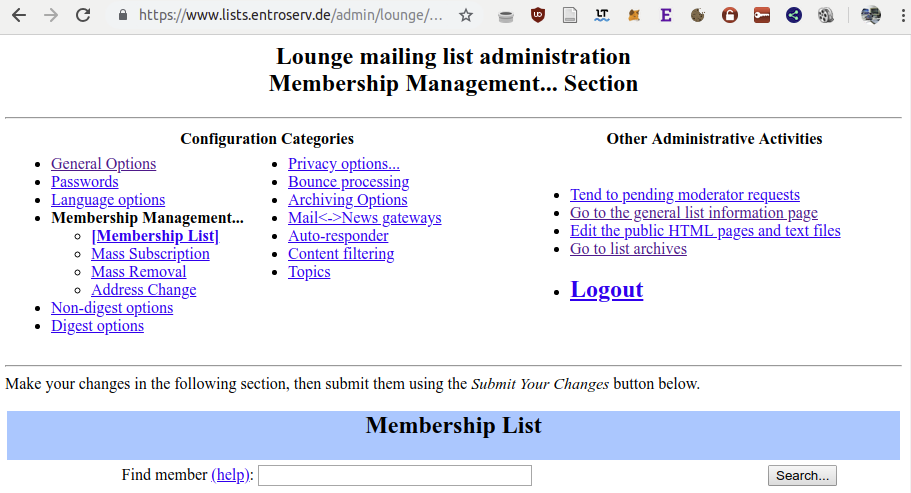
\includegraphics[width=11cm]{mailmanadmin.png}\\
\end{frame}	

\subsection{Usage}
\begin{frame}[fragile]{\insertsection}{\insertsubsection}
	%\vspace{-0.5cm}
	UI of Spamfilter \emph{Rspamd}
	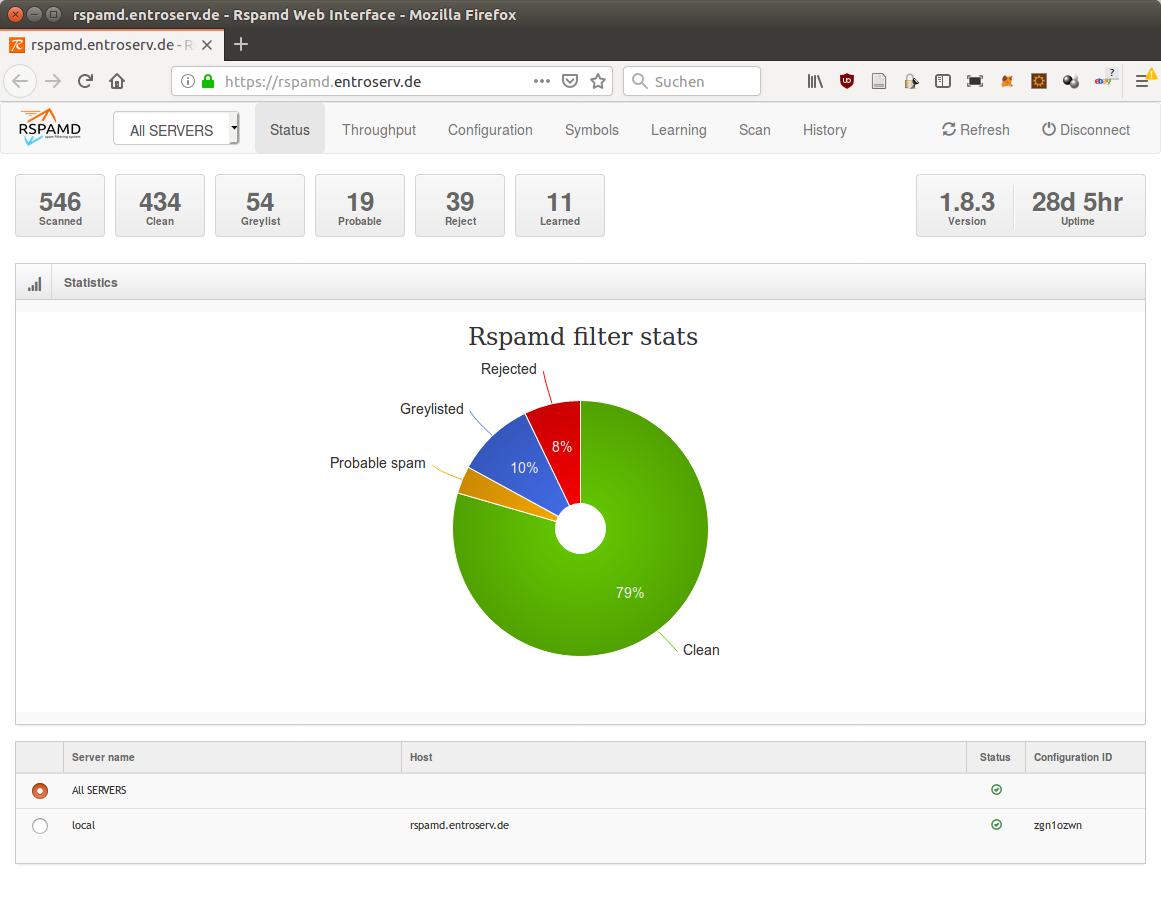
\includegraphics[width=9cm]{rspamdgui.png}\\
\end{frame}	

\begin{frame}[fragile]{\insertsection}{\insertsubsection}
	%\vspace{-0.5cm}
	\emph{Rspamd} learns Spam and Ham
	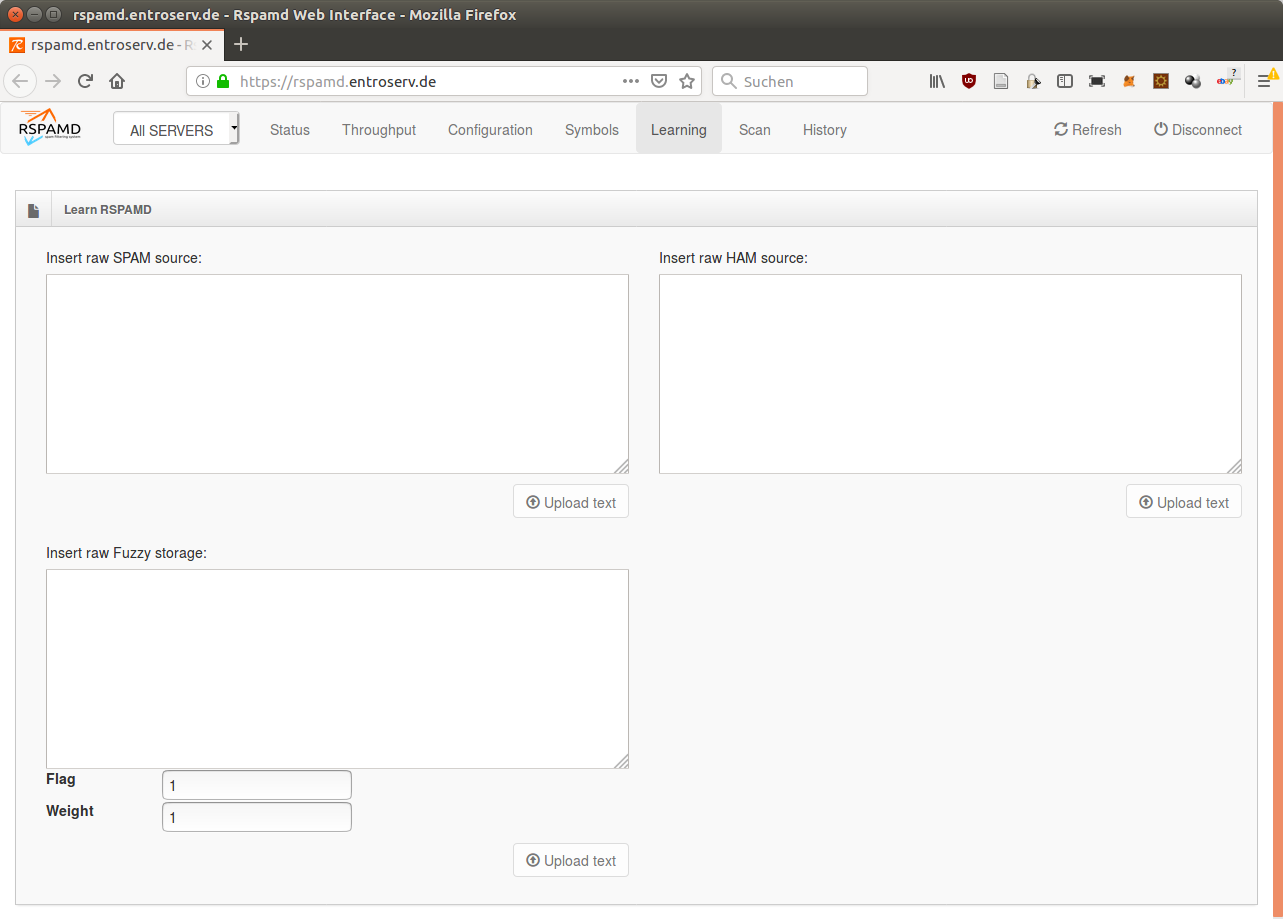
\includegraphics[width=9cm]{rspamdguilearn.png}\\
\end{frame}	

\begin{frame}[fragile]{\insertsection}{\insertsubsection}
	%\vspace{-0.5cm}
	\emph{Rspamd} learns Spam and Ham from Thunderbird
	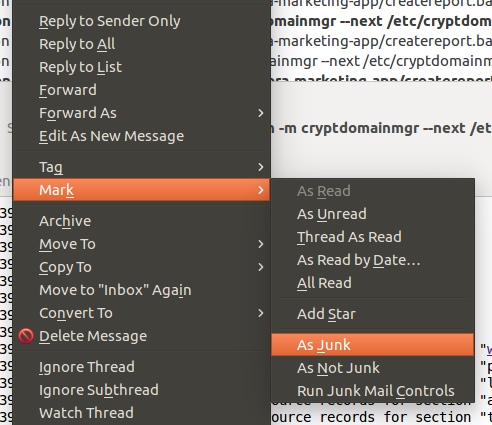
\includegraphics[height=7cm]{TBlearn.png}\\
\end{frame}	

\begin{frame}[fragile]{\insertsection}{\insertsubsection}
	%\vspace{-0.5cm}
	Signature added automatically (only tine20 and exchange)
	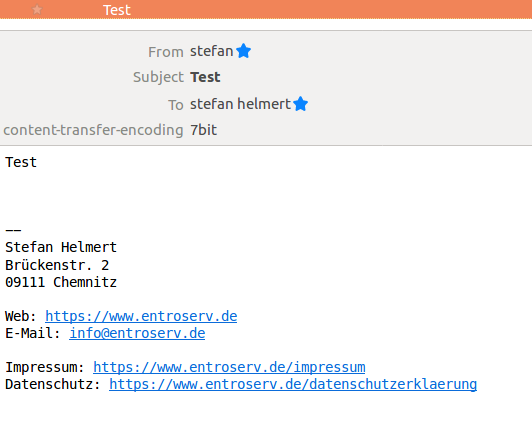
\includegraphics[height=7cm]{signature.png}\\
	Possible with IMAP?
\end{frame}

\begin{frame}[fragile]{\insertsection}{\insertsubsection}
	%\vspace{-0.5cm}
	Adminpanel of Grav CMS
	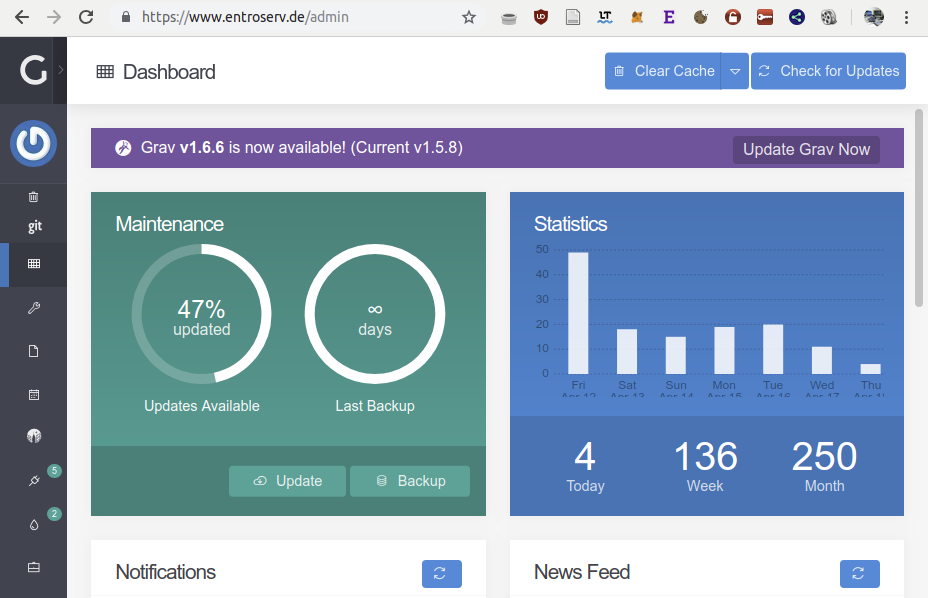
\includegraphics[height=7cm]{Grav.png}\\
\end{frame}

\begin{frame}[fragile]{\insertsection}{\insertsubsection}
	%\vspace{-0.5cm}
	How the Webpage looks like
	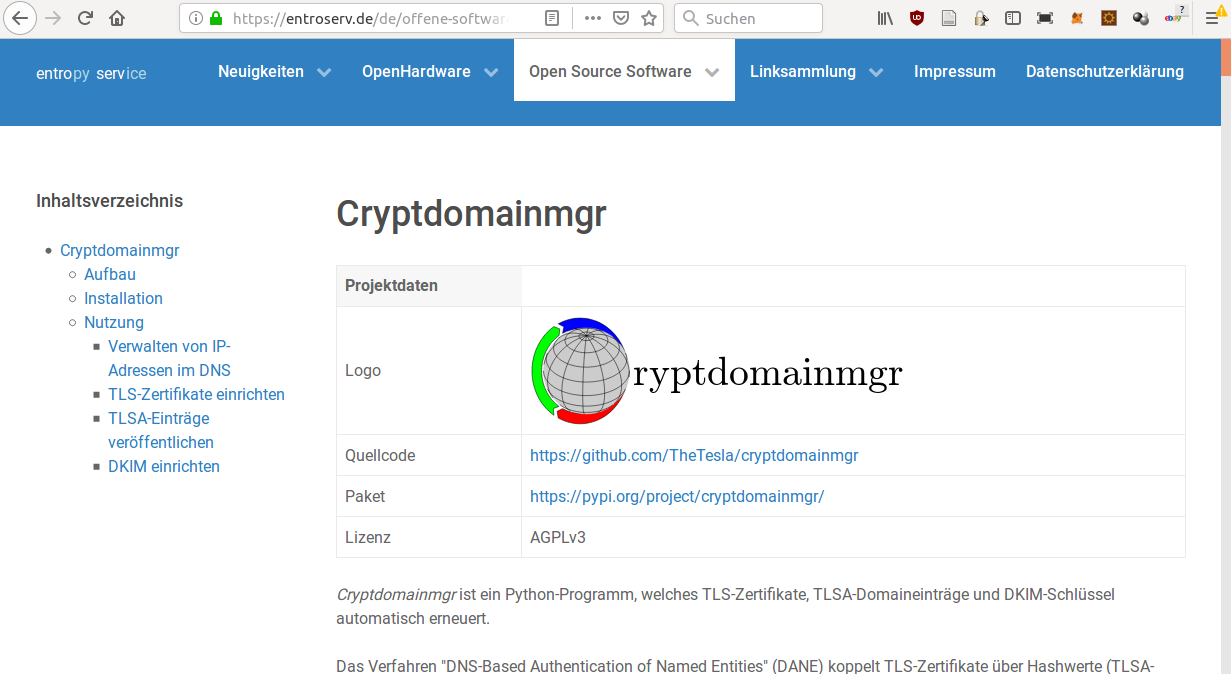
\includegraphics[height=7cm]{gravpage.png}\\
\end{frame}

\begin{frame}[fragile]{\insertsection}{\insertsubsection}
	%\vspace{-0.5cm}
	Grav TOC needs plugin
	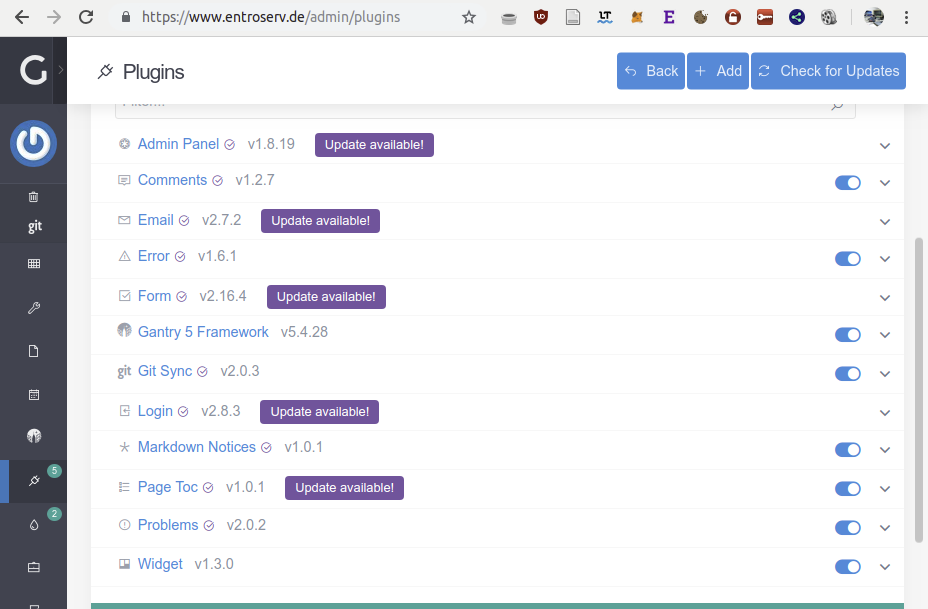
\includegraphics[width=10.5cm]{gravplugins.png}\\
\end{frame}

\begin{frame}[fragile]{\insertsection}{\insertsubsection}
	%\vspace{-0.5cm}
	Grav TOC configuration
	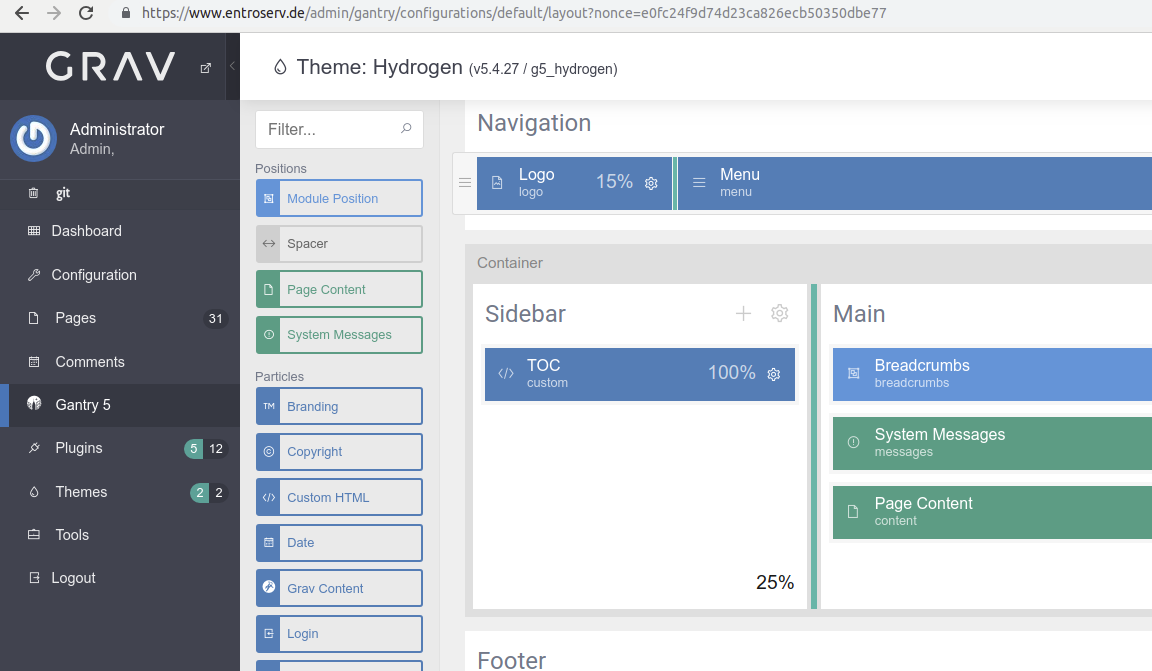
\includegraphics[width=11cm]{gravtoc.png}\\
\end{frame}

\begin{frame}[fragile]{\insertsection}{\insertsubsection}
	%\vspace{-0.5cm}
	Grav TOC configuration
	\begin{minted}[gobble=2,frame=single,linenos]{html+jinja}
		
		  
		  
			<h4>Table of Contents</h4>
			{{ toc(page.content) }}
		  
		
	\end{minted}
\end{frame}

\section{ToDo}
\section{Thanks}
\begin{frame}[fragile]{\insertsection}{\insertsubsection}
	%\vspace{-0.5cm}
	\begin{itemize}
		\item LDAP
		\item Client certificate authentication
		\item CalDav to Grav CMS events calendar
		\item Sieve, CalDav, CardDav autoconfig
		\item IMAP signature preview (if possible)
		\item Mailman tine20 integration
		\item ERP integration (also with GravCart)
	\end{itemize}
\end{frame}

\section{Thanks}
\begin{frame}[fragile]{\insertsection}{\insertsubsection}
	%\vspace{-0.5cm}
	\textbf{Thomas Leister} -- Mailserver-Howto
	\url{https://thomas-leister.de/mailserver-debian-stretch/}
\end{frame}

\section{Discussion}
\begin{frame}[fragile]{\insertsection}{\insertsubsection} % fragile: no indentation allowed
  \Huge{???}	
\end{frame}	

\end{document}





\grid
\grid
